\documentclass{article}
\begin{document}
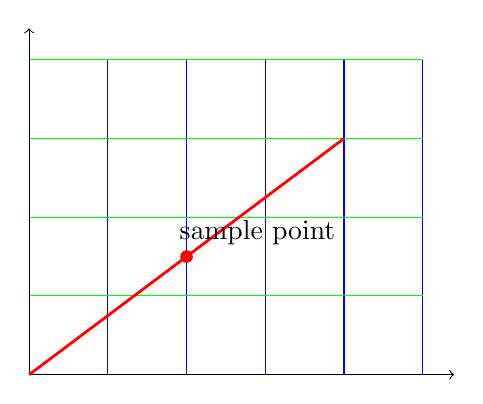
\begin{tikzpicture}
\draw[blue] (0,0) -- (0,4);
\draw[blue] (1,0) -- (1,4);
\draw[blue] (2,0) -- (2,4);
\draw[blue] (3,0) -- (3,4);
\draw[blue] (4,0) -- (4,4);
\draw[blue] (5,0) -- (5,4);
\draw[green] (0,0) -- (5,0);
\draw[green] (0,1) -- (5,1);
\draw[green] (0,2) -- (5,2);
\draw[green] (0,3) -- (5,3);
\draw[green] (0,4) -- (5,4);
\draw[->] (0,0) -- (5.4,0);
\draw[->] (0,0) -- (0,4.4);
\draw[red,line width=1pt] (0,0) -- (4,3);
\fill[red] (2,1.5) circle (0.08);
\node at (2.9,1.8) {sample point};
\end{tikzpicture}
\end{document}
